\chapter{Nozzle and Chamber Geometry (S05) and the Rao/MOC Contour Solver (S06)}\label{ch:s05-s06}

\lead{Where the engine first acquires a shape.}
Stages S05 and S06 share one block of \code{raosim/run_nozzle.py} (lines 4442--4896). S05, the default, builds
the supersonic bell from Rao thrust-optimized parabola (TOP) chart angles and a quadratic B\'ezier curve, then
assembles the convergent section and combustion chamber around one shared throat contract. S06 replaces only the
bell, and only under \code{--contour-method}~\texttt{rao-bvp}, with a finite-dimensional Rao variational
boundary-value problem (BVP) solved on a method-of-characteristics (MOC) net; the S05 chamber and geometry gates
run afterwards either way. S06 also owns the forward MOC analysis code, the port of the NASA/Johns Hopkins
University (JHU) \code{MOC_Grid_BDE} program, and the domain scans used by the multidisciplinary design
optimization (MDO) post-solve validator.

\caution{The working tree on 5 November 2026 carries an \emph{uncommitted} S05 chart change:
\code{raosim/rao_top_chart.py} is untracked and \code{raosim/nozzle_geometry.py} is modified (+53/$-$85 lines).
The angles are now a reviewer digitization of NASA SP-125 Figure 4-14 over $\varepsilon = 5$--$50$ (HEAD started
at 4 and carried an open note that its values disagreed with the SP-125 worked example), the lookup refuses every
out-of-chart point, and the reference cone length follows SP-125 Eq.~4-7 with throat rounding. Verified effects:
an out-of-chart B\'ezier run ends in an uncaught \texttt{ValueError} (exit 1) before the export gate, which is
what happens to \code{examples/cli/test_13kn_sealevel_regen_allstl.args} and
\code{examples/cli/test_13kn_movable_pintle.args} ($\varepsilon = 4.524$); and 19 of the 24 failures in this
session's full non-slow test run trace to this edit (Sections~\ref{sec:s05-verification},
\ref{sec:s06-verification}).}

% ======================================================================
\section{S05: Default B\'ezier/TOP nozzle contour, throat and chamber geometry}\label{sec:s05}
\stagetag{S05} \quad nozzle-and-chamber-geometry

\subsection{Role in the data flow and call site}

S05 runs after performance sizing (S04) has fixed the throat radius $R_t$, the ideal and delivered thrust
coefficients and the resolved ratio of specific heats $\gamma$. Inside \code{raosim.run_nozzle.main}:

\begin{enumerate}
  \item \code{_solve(args)} (\code{run_nozzle.py:1464}, called at \code{:4452}) handles the default
  \code{--contour-method}~\texttt{bezier} (\code{:2828}). It calls \code{nozzle_geometry.bell_nozzle_contour}
  (\code{nozzle_geometry.py:127}), re-labels it via \code{add_contour_reliability_metadata} under a
  frozen-variable-$c_p$ expansion, and wraps it in \code{_TrustedTopSolution} (\code{run_nozzle.py:1403}), a
  read-only adapter that presents it as a converged BVP solution with zero residuals and the
  quasi-one-dimensional (Q1D) ideal $C_F$.
  \item The gate block (\code{:4453-4840}) evaluates the solver gates; for B\'ezier only the chart-domain gate
  decides export (\code{:4806-4816}).
  \item The chamber block (\code{:4841-4896}) builds \code{ThroatGeometrySpec} and calls
  \code{auto_shoulder_factor} (\code{chamber_geometry.py:112}) under \code{--shoulder-sizing}~\texttt{auto},
  \code{chamber_contour} (\code{:138}) and \code{full_engine_contour} (\code{:440}). A \texttt{ValueError} from
  the builder, or any failure from \code{failed_thrust_chamber_geometry_checks} (\code{:432}), returns exit 2
  with no artifacts.
\end{enumerate}
One input arrives earlier: in the S03 block, \code{--cd-target} sets $R_u$ by inverting the Hall discharge
coefficient (\code{run_nozzle.py:4285-4304}), recording the source as \code{cd_target_hall_sp8120} or
\code{cd_target_hall_repository_extension}.

\needspace{8\baselineskip}
\subsection{Inputs and outputs}

\begingroup\small
\begin{longtable}{@{}P{0.34\linewidth}P{0.15\linewidth}P{0.44\linewidth}@{}}
\toprule
\textbf{Flag} & \textbf{Default} & \textbf{Use in S05} \\ \midrule
\endhead
\code{--contour-method} & \texttt{bezier} & S05 (\texttt{bezier}) or S06 (\texttt{rao-bvp}) \\
\code{--epsilon}, \code{--length-pct} & 10, 80 & chart point; exit radius $R_e=\sqrt{\varepsilon}\,R_t$ \\
\code{--allow-chart-extrapolation} & off & diagnostic out-of-chart export (inert today, Section~\ref{sec:s05-maturity}) \\
\code{--ru-factor} or \code{--cd-target} & 1.5 or none & $R_u/R_t$ directly, or from a target inviscid $C_d$ \\
\code{--allow-throat-radius-extension} & off & \code{--cd-target} range 0.6--1.5 widened to 0.6--2.0 \\
\code{--rd-factor}, \code{--convergent-angle} & 0.382, 45 deg & $R_d/R_t$ and shared half-angle $\alpha$ \\
\code{--l-star}, \code{--contraction-ratio} & 1.0 m, 2.5 & $L^*$ volume target, $A_c/A_t$ \\
\code{--shoulder-sizing}, \code{--shoulder-fill-fraction}, \code{--shoulder-radius-factor} & \texttt{auto}, 0.8, none & geometric shoulder closure; explicit $R_s/R_t$ only in \texttt{scalar} mode (legacy 0.25 if omitted there) \\
\code{--minimum-cylindrical-length} & none ($10^{-6}$ m floor) & lower bound on the cylinder \\
\bottomrule
\end{longtable}
\endgroup

\textbf{Outputs.} \code{full_engine_contour} returns one meridian from injector face to nozzle exit (with
\code{chamber}, \code{nozzle}, \code{geometry_checks}) for S07, S11 and S12.
\code{summary.json} receives \code{reliability}, \code{contour_reliability}, \code{thrust_closure},
\code{throat_geometry} (with \code{discharge_coefficient_hall}) and \code{chamber}
(\code{run_nozzle.py:4899-4966}), plus \code{hardware_qualified=False} (\code{:4968}). The first files
written are \code{contour.csv} (header \code{x_m,r_m}) and \code{profile.png} (\code{:5042-5052}). For
B\'ezier, \code{contour_audit_basis} is \code{same_quasi_1d_model}: this path never analyses the flow in the
bell it exports.

\needspace{9\baselineskip}
\subsection{Modules}

\begingroup\small
\begin{longtable}{@{}P{0.29\linewidth}P{0.06\linewidth}P{0.58\linewidth}@{}}
\toprule
\textbf{File} & \textbf{Lines} & \textbf{Role} \\ \midrule
\endhead
\code{raosim/nozzle_geometry.py} & 403 & TOP bell (two arcs, quadratic B\'ezier); chart lookup with domain refusal; dispatch of the S06 methods \\
\code{raosim/rao_top_chart.py} & 16 & $\theta_N,\theta_E$ tables from SP-125 Fig.~4-14 plus \code{EVIDENCE} (untracked) \\
\code{raosim/throat_geometry.py} & 134 & shared \code{ThroatGeometrySpec}; Hall leading-order $C_d$ and inverse \\
\code{raosim/chamber_geometry.py} & 481 & chamber meridian; $L^*$-exact volume; full-contour assembly and hard checks \\
\code{raosim/validation.py} & 399 & design-status labels, hardware note, reliability metadata, design gates \\
\bottomrule
\end{longtable}
\endgroup

\subsection{What the header comments establish}

\textbf{Nozzle contour (\code{nozzle_geometry.py}).} The header defines the three-section TOP contour: an
upstream arc ($R_u = 1.5R_t$), a downstream arc ($R_d = 0.382R_t$) and a quadratic B\'ezier ``canted
parabola'' from the inflection point $N$ to the exit $E$. It cites NASA SP-125 Figure~4-14, Eq.~4-7 and worked
example~4-2 (PDF pp.~100, 107), with SP-8120 Figure~5 and \S2.1.2.1.2 (PDF p.~29) as a conceptual cross-check,
and states that the originating Rao (1960) chart paper ``is not held; no inspection claimed''. The code
implements
\begin{align}
N &= \bigl(R_d\sin\theta_N,\; R_t + R_d(1-\cos\theta_N)\bigr), \qquad E = (L_n,\; \sqrt{\varepsilon}\,R_t),\\
L_n &= \frac{L_\%}{100}\cdot\frac{R_e - R_t + R_d(\sec 15^\circ - 1)}{\tan 15^\circ},\qquad
\mathbf{B}(t) = (1-t)^2 N + 2t(1-t)\,P_1 + t^2 E ,
\end{align}
where $P_1$ is the intersection of the tangents at $N$ and $E$ (slopes $\tan\theta_N$, $\tan\theta_E$); parallel
tangents are rejected. The \code{_full_cone_length} docstring (\code{:97}) notes that $R_d = 0$ recovers the
sharp-corner length, ``not the source's rounded-throat length''.

\textbf{Chart provenance (\code{rao_top_chart.py}).} The angles are ``reviewer digitizations, not
source-printed numerical tables''; the printed worked point (SP-125 PDF p.~107) is kept exactly. The
\code{EVIDENCE} record (chart \code{sp125-fig4-14:v2}) names the digitization file
\code{knowledge/workflows/results/agentic-2026-10-16/p1/sp125_fig4_14_digitized.json}, whose SHA-256 was
recomputed here and matches. It records a reading uncertainty of 0.3 deg (0.6 deg near
$\varepsilon = 5$--$6$); interpolation error between knots \code{NOT_ESTABLISHED}; the worked point $(14, 80)$
set to 27.4/9.8 deg over the measured 27.36/9.64 deg; a cumulative-minimum regularization that hides exit-angle
fluctuations $\le 0.16$ deg above $\varepsilon = 25$; no extrapolation; physical validation
\code{NOT_ESTABLISHED}; and SP-8120 Fig.~5b agreeing in trend but differing by up to about 1.5 deg, not averaged
in. \code{lookup_angles} (\code{:47}) interpolates bilinearly on $\varepsilon\in\{5,6,8,10,14,15,20,\dots,50\}$
by $L_\%\in\{60,\dots,100\}$ and raises outside the grid; at $(10, 80)$ it returns 25.74/10.49 deg, where the HEAD
table gave 30.0/15.5 deg.

\textbf{Throat contract (\code{throat_geometry.py}).} \code{SP8120_UPSTREAM_RADIUS_RATIO_BOUNDS} $= (0.6, 1.5)$
is ``NASA SP-8120's cited constant-efficiency design range''; \code{REPOSITORY_UPSTREAM_RADIUS_RATIO_EXTENSION_BOUNDS}
$= (0.6, 2.0)$ ``must not be labelled SP-8120''. The discharge coefficient is the Hall leading term and its
inverse,
\begin{equation}
C_d \simeq 1 - \frac{\gamma+1}{96}\left(\frac{R_t}{R_u}\right)^{2},\qquad
\frac{R_u}{R_t} = \sqrt{\frac{(\gamma+1)/96}{1-C_d^{*}}},
\end{equation}
where the inverse returns the lower bound when that already suffices and rejects a $C_d^*$ above the upper-bound
capability. \code{full_engine_contour} refuses to join a chamber and nozzle with different specifications.

\textbf{Chamber (\code{chamber_geometry.py}).} The meridian runs injector face, cylinder of radius
$R_c = \sqrt{A_c/A_t}\,R_t$, shoulder fillet $R_s$, cone at $\alpha$, upstream arc $R_u$, throat. The cylinder
length is bisected until the exact revolved-polyline volume equals $L^*A_t$, and the auto shoulder takes a
fraction $f$ (default 0.8) of the largest fillet that keeps a straight cone:
\begin{equation}
V = \sum_k \frac{\pi}{3}\,\Delta x_k\left(r_k^2 + r_k r_{k+1} + r_{k+1}^2\right) = L^* A_t,
\qquad
R_s = f\,\frac{R_c - R_t - R_u(1-\cos\alpha)}{1-\cos\alpha}.
\end{equation}
Geometry that cannot hold the volume is rejected rather than given an invented cylinder; the closure rests on
SP-8120 \S2.1.1 (throat flow is independent of geometry more than about $1R_t$ upstream).
\code{injector_to_throat_length} is kept separate from $L_c$ for the spray, residence-time and acoustic models.
In the fresh 13 kN run ($L^*$ = 1.0 m, $A_c/A_t$ = 3.0) the auto shoulder gave $R_s/R_t = 0.80$, a 0.302 m
cylinder and a frustum volume within $7\times10^{-14}$ of $L^*A_t$.
\code{HARD_THRUST_CHAMBER_GEOMETRY_CHECKS} (\code{:421}) lists seven checks: axial monotonicity, a watertight
seam within $10^{-10}$ m, position continuity, slope continuity (every join $\le 1$ deg), volume within
$10^{-8}$ relative, a positive minimum cylinder, and a wall offset free of self-intersection.

\textbf{Labels and gates (\code{validation.py}).} The checks ``are intentionally conservative. Passing them
means the generated nozzle is suitable for downstream design review, not qualified for hardware.''
\code{DESIGN_STATUS_BY_METHOD} maps \texttt{bezier} to \code{preliminary_top_geometry}, \texttt{moc} to
\code{experimental_moc_geometry}, \texttt{rao} to \code{experimental_variational_geometry} and
\code{rao_variational_moc} to \code{experimental_rao_variational_moc_bvp}, always with
\code{hardware_qualified=False} and the note ``Requires independent CFD, thermal/structural analysis,
manufacturing review, inspection, and hot-fire evidence''. \code{add_contour_reliability_metadata}
(\code{:90}) warns on an exit-radius error above 0.5\%, exit Mach more than 25\% from the area--Mach value, or
exit angle above 10 deg. \code{evaluate_design_gates} (\code{:161}) adds curvature, wall-pressure, separation
and CAD checks and the status check ``Only the Rao/TOP Bezier path is currently treated as the trusted
baseline''; it is called by \code{design.design_nozzle_v2}, \code{design.design_nozzle} and the legacy
\code{main.py}, not by the \code{lrekit}/\code{raosim} runner.

\needspace{8\baselineskip}
\subsection{Governing documents}

\begingroup\small
\begin{longtable}{@{}P{0.40\linewidth}P{0.12\linewidth}P{0.08\linewidth}P{0.31\linewidth}@{}}
\toprule
\textbf{Path} & \textbf{Type} & \textbf{Status} & \textbf{Content} \\ \midrule
\endhead
\code{docs/subsystems/S05-nozzle-and-chamber-geometry/shoulder_radius_design_basis.md} & subsystem basis & active & $R_u$ ($C_d$, heat flux) versus $R_s$ (subsonic, manufacturing); Tier 1 and \code{--cd-target} landed; Tier 2 open \\
\code{docs/literature/chamber_design_literature.md} & literature & active & $L^*$, contraction, half-angle and arc rules mapped to SP-125/SP-8120; acquisitions SP-8089, SP-8113, SP-194 \\
\code{docs/data/rao_nozzle.csv} & data & stub & orphan 200-point contour; no provenance or reader \\
\code{docs/archive/rao_nozzle_profile.csv} & data & stub & stray \code{main.py} output \\
\bottomrule
\end{longtable}
\endgroup

\textbf{Doc versus code.} The design-basis memo is internally inconsistent: \S2 quotes SP-8120 for ``$R_u/R_t$
values from 1.5 down to 0.6'', while \S4A and \S5 give $0.6 \le R_u/R_t \le {\sim}2$ as the SP-8120 range. The code
treats 1.5 as the SP-8120 bound and 2.0 as a flagged repository-only extension; the code governs.

\subsection{Verification}\label{sec:s05-verification}

Status comes from this session's full non-slow run on the working tree (\code{.venv-jax}; 2,832 passed, 24
failed, 1 skipped, 27 deselected, the 27 being exactly the \texttt{slow}-marked items). Counts are collected items.

\begingroup\small
\begin{longtable}{@{}P{0.33\linewidth}P{0.63\linewidth}@{}}
\toprule
\textbf{Test} & \textbf{What it pins; status on 5 Nov 2026} \\ \midrule
\endhead
\code{tests/test_chamber_geometry.py} (20) & analytic shoulder cap; auto fraction; Hall $C_d$ and inverse; shared spec; $L^*$ volume over $3\times3$ ($L^*$, $A_c/A_t$); exact frustum volume; offset gate when an offset is supplied; infeasible chamber rejected. Pass. \\
\code{tests/test_nozzle_geometry.py} (12), \code{tests/test_run_nozzle.py} chart test & arc-to-bell $C^0$/$G^1$ continuity, exit radius, monotone bell; CLI exit 2 out of chart. \textbf{Five fail}: \code{test_known_point} expects about 30 deg; \code{test_bell_length} expects the sharp-corner length (0.12912 against 0.12992 m); two query out of chart ($\varepsilon = 60$, and $\varepsilon = 4$ in a sweep) and hit the \texttt{ValueError}; the CLI test gets exit 1 with a traceback. \\
\code{tests/test_design_workflow.py} (11), \code{tests/test_design_v2.py} (56) & design API, gates, STEP export. \textbf{Four fail}: three build a B\'ezier at $\varepsilon = 4$; the $\varepsilon = 60$ block raises instead of returning a blocked result. \\
\code{tests/test_benchmarks.py} (7) & external-geometry benchmarks. \textbf{Two fail}: the LEA TOP (Schomberg 2014) B\'ezier case misses \code{length_over_rt} (15.045 against 15.0, tolerance 0.02) because its $L_\%$ was derived with the sharp-corner cone; its CLI wrapper fails with it. \\
\code{tests/test_mdo_engine.py}, \code{tests/test_mdo_bounds.py} & S13 copies of the chart. \textbf{Four fail}: the JAX chart and $\varepsilon$ bound now start at 5. \\
\bottomrule
\end{longtable}
\endgroup

No test imports \code{raosim/rao_top_chart.py}, pins its \code{EVIDENCE} record, or pins the SP-125 worked point
$(14, 80) \to 27.4/9.8$ deg.

\subsection{Maturity, limitations and known defects}\label{sec:s05-maturity}

\begin{itemize}
  \item \textbf{Label inconsistency.} Design status \code{preliminary_top_geometry} and registry level
  \code{benchmark_screened_not_hardware_validated} (\code{model_registry.py:451}) disagree with the reliability
  \code{benchmark_validated} that \code{_TrustedTopSolution} assigns and \code{summary.json} reports; the chart
  record itself says physical validation is not established.
  \item \textbf{Broken chart-domain handling (working tree).} \code{lookup_angles} raises before
  \code{rao_chart_extrapolated} can be set, so that flag, its warning, the \code{geometric_approximation} branch
  of \code{_TrustedTopSolution} and \code{--allow-chart-extrapolation} are dead code paths.
  \item \textbf{Not Rao's shock-free contour.} On chart B\'ezier walls the bounded MOC net stops with
  \code{rrc_coalescence}, an internal compression shock (Section~\ref{sec:s06-bounded}); S05 reports Q1D $C_F$.
  \item \textbf{Hall $C_d$ is reported, not applied.} \code{engine.py} has no discharge coefficient, so the
  throat is sized on geometric area; \code{--cd-target} changes only $R_u$.
  \item \textbf{Vacuous wall-offset gate in the CLI.} \code{full_engine_contour} calls
  \code{thrust_chamber_geometry_checks} without \code{offset_distance}, so \code{offset_self_intersection_free}
  passes trivially (the fresh 13 kN summary records \code{"offset_checked":false}); only \code{design.py:1754}
  supplies a wall thickness.
  \item \textbf{Length-convention drift.} Only the CLI B\'ezier uses the rounded-throat cone. The sharp-corner
  $(R_e - R_t)/\tan 15^\circ$ remains in \code{rao_variational} (\code{_target_length} \code{:2501},
  \code{:2081}, \code{:6882}), \code{rao_existence_scan.target_length} (\code{:1532}),
  \code{rao_optimizer._full_cone_length} (\code{:53}), \code{mdo/grid.py:381}, \code{jax/design_opt.py:347} and
  \code{nozzle_comparison.py:169}. The difference is 0.62\% at $\varepsilon = 10$ and 1.2\% at
  $\varepsilon = 4.524$: the fresh \texttt{rao-bvp} wall ends at $x_E = 104.10$ mm (sharp-corner value) where
  a B\'ezier with the same flags would end at 105.35 mm.
  \item \textbf{Source mismatch.} The registry source for \code{nozzle.rao_top_bezier} is SP-8120
  (\code{19770009165.pdf}); the chart is digitized from SP-125 (\code{19710019929.pdf}).
  \item \textbf{Generic chamber defaults.} $L^*$ = 1 m, contraction ratio 2.5 and $\alpha$ = 45 deg are generic
  preliminary values; Tier-2 optimization of $R_s$ is not implemented.
\end{itemize}

\subsection{Developer notes}

\begin{itemize}
  \item \emph{Chart data}: edit \code{raosim/rao_top_chart.py} and its \code{EVIDENCE} record; then update
  \code{tests/test_nozzle_geometry.py}, the 30/15.5 deg docstrings in \code{tests/test_rao_chart_benchmark.py},
  \code{RAO_CHART_THETA_SEED_SOURCE_ID} in \code{rao_existence_scan.py} and the S13 bound tests
  (\code{mdo/grid.py} imports the tables and follows automatically).
  \item \emph{Out-of-chart behaviour and reference length}: catch the lookup error in \code{run_nozzle._solve}
  and \code{design._build_v2_contour}; introduce one shared cone-length helper.
  \item \emph{Throat, chamber, labels}: \code{throat_geometry.py} (a $C_d$ that should change mass flow must also
  reach \code{engine.compute_engine_performance}); \code{chamber_geometry.py} and
  \code{HARD_THRUST_CHAMBER_GEOMETRY_CHECKS} (pass \code{offset_distance} from the CLI if the offset check should
  bind); \code{validation.py}, noting that the chart path's CLI reliability is set in \code{_TrustedTopSolution}.
\end{itemize}

% ======================================================================
\section{S06: Opt-in Rao variational / method-of-characteristics BVP contour}\label{sec:s06}
\stagetag{S06} \quad rao-moc-bvp-contour

\subsection{Role in the data flow and call site}

With \code{--contour-method}~\texttt{rao-bvp}, \code{_solve} (\code{run_nozzle.py:1489-1508}) builds a
\code{RaoSolverConfig} and calls \code{rao_variational.solve_rao_bvp} (\code{rao_variational.py:5901}). The CLI
fixes \code{wall_method="bde"}, \code{kernel_d_fraction_max=0.7} and \code{physics_weight=1.0}; flags supply the
rest (defaults): \code{--backend} (\texttt{jax}), \code{--n-control}/\code{--n-kernel} (24), \code{--max-nfev}
(4000), \code{--theta-b-guess} (30 deg), \code{--kernel-dtheta-limit-deg} (0.25 deg) and
\code{--kernel-massflow-rel-tol} (0.02). The \code{RaoSolution} then passes the S05 gate block with every solver
gate active, and the S05 chamber is attached. S06 is also reached from the opt-in MDO post-solve validator
``B3'' (\code{mdo/contour_validation.py}: \texttt{bde} wall at $24\times24$, refined at $32\times32$, 0.25 deg
kernel step, reading the ``B5'' domain artifact through \code{RaoConvergenceDomain}, which
\code{mdo/execute.py:503} also loads); from the MDO branches, which accept \code{rao-bvp} only with
\code{--mdo-export} and \code{--cad}~\texttt{none} (\code{run_nozzle.py:1866}); and from \code{bell_nozzle_contour}
methods \code{'moc'}, \code{'rao'}, \code{'rao_variational_moc'}, \code{benchmarks.py} and the legacy
\code{main.py}.

\subsection{Inputs and outputs}

\textbf{Inputs} are $R_t$, $\varepsilon$, $\gamma$, $p_a/p_0$, $L_\%$, $R_u/R_t$, $R_d/R_t$ and the solver flags under
\code{RAO_MOC_ASSUMPTIONS} (axisymmetric, inviscid, isentropic, constant-$\gamma$); the frozen-variable-$c_p$
expansion is refused with \code{rao-bvp} (\code{run_nozzle.py:3852}). The $\theta_B$ secant starts from
\code{--theta-b-guess} (\code{:2769}); the chart design angles used for the station $N$ and the
\texttt{coupled}/\texttt{legacy} wall slopes come from \code{_design_angles_rad} (\code{:1721}), which catches
\emph{any} \code{lookup_angles} exception and falls back to the guess and half of it (30/15 deg by default), so the
13 kN \code{rao-bvp} example still runs at $\varepsilon = 4.524$.

\textbf{Outputs.} The \code{RaoSolution} carries residuals, a reliability level, $\theta_N$ (identically the
kernel arc-end angle $\theta_B$), $\theta_E$, and $C_F$ from the full C-D-E control-surface integral when that
surface is complete; \code{construction_diagnostics} hold the net report, BDE integrity, numerical policy,
export diagnostics, \code{benchmark_validation} and \code{nasa_reference_validation}.
\code{RaoSolution.to_contour_dict} (\code{:1140}) refuses export unless the Rao (1999) Eq.~(5) verdict is valid,
and bridges the throat to the wall's first station with a Hermite cubic (\code{throat_bridge}) because the BDE
wall does not start on the $R_d$ arc at its own slope. It does \emph{not} call
\code{add_contour_reliability_metadata}, so the CLI BVP contour has \code{reliability} and
\code{hardware_qualified=False} but no \code{design_status}. On disk the stage adds
\code{contour_moc_crossings.csv} when crossings were sampled (\code{run_nozzle.py:5053}); in memory,
\code{bde_artifacts} feed the five S12 construction diagrams and enable \code{--flowfield}/\code{--animate}, both
refused for B\'ezier (\code{:3901}).

\needspace{9\baselineskip}
\subsection{Modules}

\begingroup\small
\begin{longtable}{@{}P{0.29\linewidth}P{0.06\linewidth}P{0.58\linewidth}@{}}
\toprule
\textbf{File} & \textbf{Lines} & \textbf{Role} \\ \midrule
\endhead
\code{raosim/rao_variational.py} & 7083 & BVP configuration, residual stack, backends, wall construction (\texttt{bde}, \texttt{coupled}, \texttt{legacy}), audits, reliability ladder; legacy \code{rao_variational_contour} \\
\code{raosim/nasa_moc.py} & 3589 & port of NASA/JHU \code{MOC_GridCalc_BDE.cpp}: TT$'$ line, kernel march, mass flow, \code{find_point_e}, \code{calc_lrc_de}, \code{set_theta_b}, BDE region, full-surface thrust \\
\code{raosim/rao_existence_scan.py} & 2926 & solver-independent D-attachment scans; typed, hash-pinned $\varepsilon\times L_\%$ domain (B5) \\
\code{raosim/moc.py} & 890 & Anderson-form unit processes; \code{solve_flowfield}; deprecated front march \\
\code{raosim/moc_bounded.py} & 763 & bounded RRC-by-RRC analysis net on the NASA/JHU topology; exit-plane crop \\
\code{raosim/rao_optimizer.py} & 433 & experimental direct wall-shape optimizer (not CLI-reachable) \\
\code{raosim/moc_topology.py} & 305 & explicit \code{RaoTopology} (TT$'$, B, BF, D, BD, DE, E, wall streamline) \\
\code{raosim/transonic_kernel.py} & 303 & third-order Kliegel--Levine kernel with corrected NASA coefficient typos \\
\code{raosim/wall_model.py} & 173 & monotone cubic Hermite \code{SplineWall} \\
\code{raosim/rao_residuals.py} & 160 & axisymmetric C$^{\pm}$, left-Mach-line and wall-tangency residuals \\
\bottomrule
\end{longtable}
\endgroup

\needspace{12\baselineskip}
\subsection{Three ways the repository can produce a bell}

\begingroup\small
\begin{longtable}{@{}P{0.14\linewidth}P{0.26\linewidth}P{0.27\linewidth}P{0.25\linewidth}@{}}
\toprule
\textbf{Path} & \textbf{What is solved} & \textbf{Reached from} & \textbf{Status} \\ \midrule
\endhead
B\'ezier/TOP (S05) & no flow solve; chart angles plus a quadratic B\'ezier & CLI default; MDO grid (a JAX bilinear copy of the tables); design API & \code{preliminary_top_geometry}; the CLI reports \code{benchmark_validated} \\
Variational BVP & control surface DE on kernel BD; mass and length closure, algebraic stationarity, C$^+$ compatibility; wall from the BDE region & \code{rao-bvp} (\texttt{bde}); B3; \code{bell_nozzle_contour('rao_variational_moc')} (library default wall \texttt{coupled}) & experimental; per-run ladder up to \code{rao_variational_residual_solved} \\
Forward MOC + direct optimizer & bounded net of a \emph{given} wall; SLSQP or Nelder--Mead on spline radii & \code{bell_nozzle_contour('moc')}; \code{benchmarks.py}; forward audit of \texttt{coupled}/\texttt{legacy} walls & \code{experimental_moc_geometry}; optimum not benchmarked \\
Legacy variational & direct-method control surface plus a sequential MOC wall & \code{bell_nozzle_contour('rao')} & \code{experimental_variational_geometry} \\
\bottomrule
\end{longtable}
\endgroup

\begin{figure}[tbp]
\centering
\begin{tikzpicture}[
  node distance=2.4mm and 5mm,
  box/.style={draw=teal, rounded corners=2pt, fill=pale, align=left, font=\scriptsize\sffamily,
              text width=0.50\linewidth, inner sep=2.5pt},
  side/.style={draw=rulegray, rounded corners=2pt, align=left, font=\scriptsize\sffamily,
              text width=0.38\linewidth, inner sep=2.5pt},
  arr/.style={-{Stealth[length=1.8mm]}, thick, color=ink}]
\node[box] (cfg) {\textbf{run\_nozzle.\_solve} (:1464) $\to$ RaoSolverConfig: wall\_method=bde, kdf $\le$ 0.7, kernel step 0.25$^\circ$, $\dot m$ tol 2\%};
\node[box, below=of cfg] (seed) {\textbf{\_initial\_ce\_from\_kernel} (:2713): nasa\_moc.set\_theta\_b secant on $\theta_B$; calc\_lrc\_de / find\_point\_e place D on BD so DE reaches $r_E$ with $\dot m_{BD}=\dot m_{DE}$};
\node[side, right=of seed] (kern) {build\_kernel: TT$'$ from \_make\_throat\_initial\_line and kliegel\_levine($R_u$); RRC march on the $R_d$ throat arc to $\theta_B$; last RRC = BD};
\node[box, below=of seed] (pack) {\textbf{\_pack\_bvp} (:2958): $[M,\theta,r]$ on CE, $\lambda_2,\lambda_3,\log C$, kdf; blocks mass, length, moc\_cplus, ce\_geometry, regularization, penalties, algebraic\_stationarity, wall\_endpoint, wall\_tangency};
\node[box, below=of pack] (solve) {\textbf{Backend}: jax $\to$ least\_squares\_jax (:6071; Optimistix LM, autodiff Jacobian, weight ladder 1/10/30/100); numpy $\to$ SciPy least\_squares (:6079); max\_nfev $\le$ 0 $\to$ seed residual only};
\node[side, right=of solve] (tb) {solve\_theta\_b (JAX only; not set by the CLI): BD re-marched in-graph};
\node[box, below=of solve] (wall) {\textbf{Wall} (:6154): bde $\to$ \_wall\_from\_bde\_region $\to$ calc\_bde\_region; measured-mesh topology report};
\node[side, right=of wall] (cw) {coupled/legacy: SplineWall, then solve\_flowfield $\to$ march\_bounded\_net forward audit (:6199)};
\node[box, below=of wall] (aud) {\textbf{Audits $\to$ ContourReliability} (:6670): residuals, BDE integrity, Rao-1999 Eq.~(5) $dR/R \ge 0$, full C-D-E thrust sanity (5\%)};
\node[box, below=of aud] (gate) {\textbf{run\_nozzle gates} (:4453--4840): export, or exit 2 unless --allow-unconverged};
\draw[arr] (cfg) -- (seed); \draw[arr] (seed) -- (pack); \draw[arr] (pack) -- (solve);
\draw[arr] (solve) -- (wall); \draw[arr] (wall) -- (aud); \draw[arr] (aud) -- (gate);
\draw[arr, densely dashed] (kern) -- (seed); \draw[arr, densely dashed] (tb) -- (solve);
\draw[arr, densely dashed] (cw) -- (wall);
\end{tikzpicture}
\caption{Internal flow of solve\_rao\_bvp as called by the CLI. Line numbers refer to rao\_variational.py
unless noted. Unshaded boxes are sub-steps or alternatives that the CLI does not select.}
\end{figure}

\subsection{What the header comments establish}

\textbf{MOC unit processes (\code{moc.py}).} ``Layer 1 of the Rao nozzle design'' owns the Anderson-form
interior, axis and wall unit processes. With nodes ordered downstream,
\begin{equation}
\text{C}^{+}\,(\theta+\mu):\ d(\theta-\nu) = -S\,ds,\qquad
\text{C}^{-}\,(\theta-\mu):\ d(\theta+\nu) = +S\,ds,\qquad
S = \frac{\sin\theta\,\sin\mu}{r}\quad(S=0\ \text{planar}),
\end{equation}
Anderson (\emph{Modern Compressible Flow}, 3rd ed.) eqs.~11.52/11.53, ``oracle-validated 2026-06-11 against the
NASA M3.5Perf net''; the Rice NASA/JHU manual (20030067852) and SP-8120 are also cited. \code{solve_flowfield}
starts from the axis-to-wall Kliegel--Levine data line (or \code{nasa_visible_kliegel_levine} for oracle
parity); \code{approximate_starting_line} samples the throat arc and must not be used as MOC initial data. The
old \code{march_coupled_net}, whose axis and wall points ``were never parents of any later point'', is kept,
deprecated, ``for the audit trail only''.

\textbf{Bounded net (\code{moc_bounded.py}).} A forward \emph{analysis} march between the axis and a given wall
on the NASA/JHU topology (Rice manual PDF 7--9, 17; C++ \code{CalcRRCsAlongArc}, \code{CalcInteriorMeshPoints},
\code{CalcAxialMeshPoint}; Anderson \S11.5). Each right-running characteristic (RRC) is stored wall-first; interior
point $[i][j]$ is the C$^+$ of $[i+1][j-1]$ crossed with the C$^-$ of $[i-1][j]$, so the wall point is a parent,
and the axis closes each row; $i_{\text{last}}[j] = i_{\text{last}}[j-1] + \text{specialFlag}$ never shrinks except
by negative-radius truncation. Throat-arc rows reuse the NASA arc unit processes verbatim, so they equal
\code{build_kernel}. Invalid cells ``are never geometrically patched'': one half-step refinement, then a named
stop (Young 2012 eq.~3.10; Rice: refine DTHETAB). The stop reasons in code are \code{exit_reached},
\code{max_rrcs}, \code{rrc_coalescence}, \code{invalid_cell}, \code{massflow_drift}, \code{row_too_short} and
five wall-point failures. The exit plane follows NASA \code{CropNozzleToLength}.

\textbf{NASA/JHU port (\code{nasa_moc.py}).} A ``stagnation-normalised Python port'': \code{build_kernel} is
\code{CalcInitialThroatLine} plus \code{CalcRRCsAlongArc}; \code{calc_massflow_along_rrc}/\code{calc_mdot_bd} are
the annular trapezoidal mass flow; \code{find_point_e} secants the last radial step until the DE mass equals
$\dot m_{BD}$; \code{calc_lrc_de} secants D until $\theta_E - \theta_{\text{calc}}(p_E,\rho_E,M_E) = 0$;
\code{set_theta_b} secants $\theta_B$. Docstrings add that TT$'$ radii follow
$r/R_t = \sin^{1.5}\bigl(\tfrac{\pi}{2}(n-i)/n\bigr)$; that the \code{kliegel_levine} line walks subsonic points
downstream until $M \ge 1.05$ while the NASA-visible line keeps the literal $M \le 1.5$ cap loop; that the series
uses the \emph{upstream} curvature (the C++ passes \code{rUp}); and that the 0.5 deg DTHETAB default and 2\%
per-RRC mass check are ``a numerical implementation diagnostic, not a conservation law or physical limit''.

\textbf{Transonic kernel (\code{transonic_kernel.py}).} Kliegel and Levine (1969), AIAA~J. 7(7), third-order
toroidal expansion ``valid down to $R_c/R_t \sim 0.5$''. It ports NASA \code{KLThroat} (C++ 3103--3178) with
corrections: axisymmetric line 3133 (\texttt{*} to \texttt{+}, 1181 to 1881, $y^2$ to $y^3$), line 3129 (/34 to
/384) and planar line 3157 (\texttt{*} to \texttt{+}); ``Do not `fix' the comments back to literal NASA
source.'' The returned $M = \sqrt{U^2+V^2}$, with $U,V$ normalized by $a^*$, is the critical Mach number $M^*$
(finding F11); the registry note says this NASA-visible convention is kept for oracle parity.

\textbf{Topology object (\code{moc_topology.py}).} Formalizes REWRITE\_PLAN \S11.7 (TT$'$, B, BF, D, BD, DE, E,
\code{streamline_BE}, $\theta_B$, $\dot m_{BD} = \dot m_{DE}$). Once the characteristic formulation is the default,
``this field --- not \code{_construct_wall_from_ce} --- is the wall''.

\textbf{Variational BVP (\code{rao_variational.py}).} An ``experimental Rao-style variational nozzle prototype''
using the Rao/NASA thrust, mass-flow and length functionals with the ambient-pressure term, experimental ``until
published benchmarks pass''. The residual solve ``is a finite-dimensional direct method''; the Rao 1958 Nozzle-B
benchmark ``validates its published shape/integral envelope, not every internal characteristic state''; a result
is ``promoted only when its per-run BVP and MOC topology gates pass''. References: Rao (1958), a NASA TM (1990)
re-derivation, SP-8120. The body defaults to the \code{characteristic} formulation (dropping the C$^-$-along-CE
and CE-to-wall scaffold blocks), the \texttt{jax} backend and \code{angle_boundary_mode="free"} (chart angles only
seed). The valid-region test is Rao, Beck and Booth (AIAA 99-2584) Eq.~(5): predicted $dR/R \ge -10^{-9}$ on every
DE segment, with no discontinuous-exit-flow fallback. All finite thresholds sit in \code{RaoMOCNumericalPolicy},
labelled \code{repository_numerical_policy_not_physical_criterion}.

\textbf{Residuals, optimizer, scans, wall.} \code{rao_residuals._source_axisym} records the 2026-06-11 removal of a
spurious $\cos\mu/\cos(\theta\pm\mu)$ factor and of a mirrored C$^\pm$ pairing (oracle RMS $2.3\times10^{-6}$ and
$8.8\times10^{-8}$ afterwards). \code{rao_optimizer} (``Layer 2'') scores
\code{SplineWall} candidates with the bounded net, penalising coalescing candidates ``by how far the wall was
reached''; it ``is not reachable from any CLI/MDO path and its optimum has not been benchmarked''; its $\theta_N$
seed is an SP-8120 step table. \code{rao_existence_scan} ``deliberately stays out of the JAX/Optimistix/least-squares
stack'', sampling $(\theta_B, \text{kdf})$ under \texttt{smooth}, \texttt{position} and \texttt{fan} D-attachment
closures (the last a centred Prandtl--Meyer fan); its \code{scan_convergence_domain} (\code{:2472}) builds B5, where
``numerical failure remains unknown rather than being labelled physical non-existence''.
\code{SplineWall.intersect_char} still clamps its iterate (F4); the bounded net uses
\code{moc_bounded.intersect_wall_strict}, which returns \code{None} instead.

\begin{figure}[tbp]
\centering
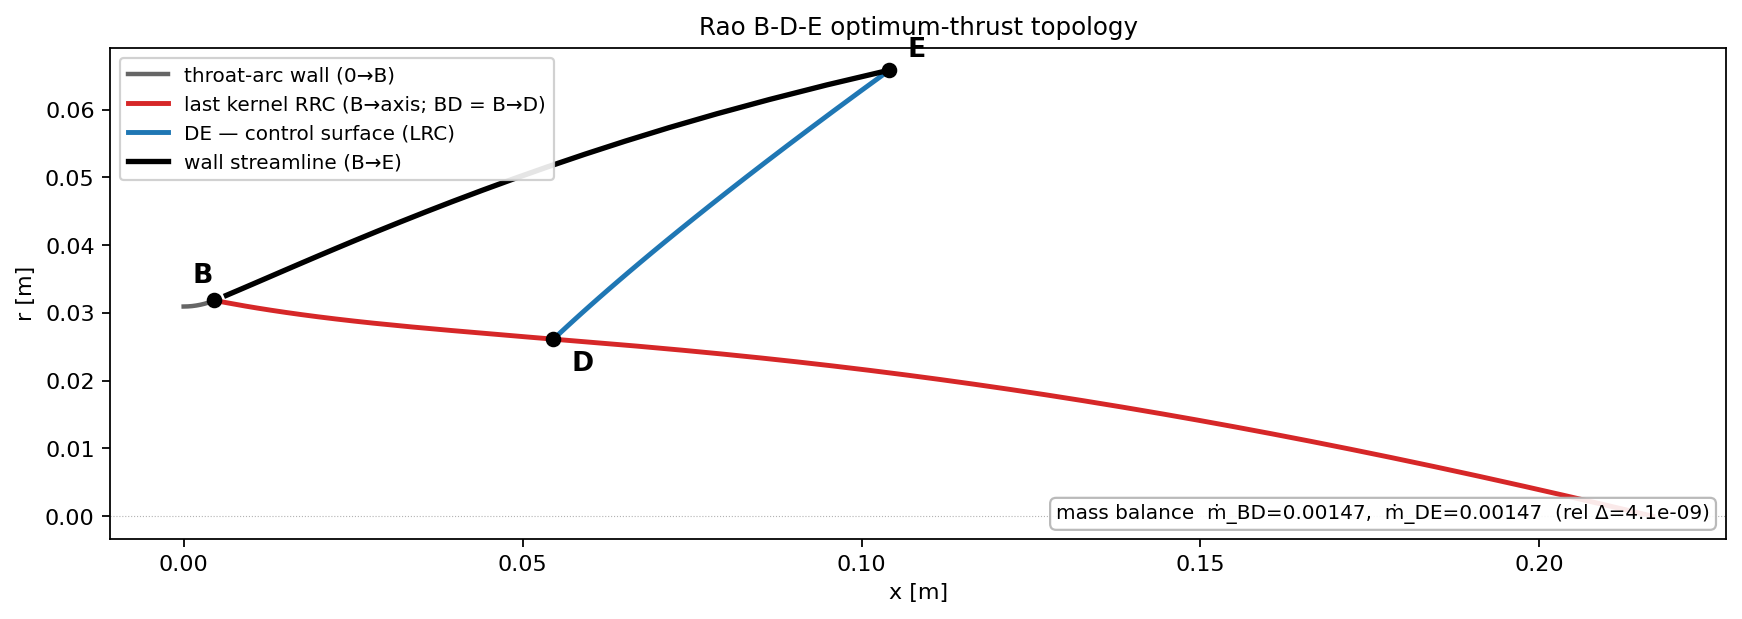
\includegraphics[width=0.76\linewidth,keepaspectratio]{figures/fresh/fresh_13kn_rao_bde_topology.png}
\caption{Rao B-D-E topology from the fresh 13 kN rao-bvp run of 5 November 2026 ($\varepsilon = 4.524$,
$L_\% = 80$, $\gamma = 1.24$, $\theta_B = 22.58$ deg): throat arc to B, last kernel RRC through D, control
surface DE, wall streamline B--E. BD and DE mass flows differ by a relative $4.1\times10^{-9}$.}
\end{figure}

\subsection{The bounded MOC net fix and compression coalescence}\label{sec:s06-bounded}

\code{docs/subsystems/S06-rao-moc-bvp-contour/MOC_MARCH_TOPOLOGY_REMEDIATION_2026-09-21.md} confirmed twelve
findings (F1--F12) against the old forward march: boundary points were never parents, so the net shrank by one
point per row and died at about 30\% of the length (F1, F2); the starting line was the wall arc (F3); every wall
point collapsed onto $N$ (F4); a two-point exit plane gave $C_F = 0.81$ where about 1.65 was expected (F6); the
tests enshrined the defect (F7). The blast radius was small: the MDO uses the B\'ezier and Q1D $C_F$, and the CLI
\code{rao-bvp} path and B3 use the \texttt{bde} wall; only the \texttt{coupled}/\texttt{legacy} forward audits,
\code{method='moc'} and \code{flow_viz} fed with those rows were affected.

Phases 0--2 landed the same day as \code{moc_bounded.py}. \textbf{Oracle A}: throat-arc rows bit-identical to
\code{build_kernel}. \textbf{Oracle B} (M3.5Perf wall, NASA-visible line, DTHETAB 0.5 deg): wall Mach RMS
$3.1\times10^{-4}$ against \code{wall.out}; axis Mach RMS $8.9\times10^{-3}$ against \code{center.out} (halving
at 0.25 deg); exit $M = 3.5009\pm0.0017$, $\theta_{\text{rms}} = 0.003$ deg; stream thrust 2517.72 against 2518.05
lbf; mass flow 35.989 against 35.998 lbm/s.

The audit also found physics: on a chart B\'ezier bell the first bell RRC crosses BD, i.e. the compression waves
coalesce into an internal shock, consistent with the TOP internal-shock literature (Hagemann 1998; Frey and
Hagemann 2000). The net stops with \code{stop_reason="rrc_coalescence"} and a \code{fold_location}; downstream,
\code{moc_bell_nozzle} exports NaN exit metrics and an incomplete \texttt{coupled}/\texttt{legacy} audit sets
\code{moc_compatibility_preserved=False}.

\caution{The remediation record and the registry place the coalescence ``about 20 mm past N at $R_t$ = 20 mm'',
measured on the HEAD chart. On the working-tree chart ($\theta_N = 25.74$ deg at $(10, 80)$),
\code{test_solve_flowfield_reports_bezier_compression_coalescence} still gets \code{rrc_coalescence}, but at
$x = 55.3$ and 51.6 mm at its two resolutions, outside its 3 mm convergence tolerance and 15--35 mm band. The
coalescence finding stands; the quoted location is stale.}

\subsection{Reliability ladder and export gates}

\code{ContourReliability} (\code{rao_variational.py:148}) orders \code{geometric_approximation} $<$
\code{moc_compatible} $<$ \code{rao_variational_residual_solved} $<$ \code{nasa_reference_matched} $<$
\code{benchmark_validated} $<$ \code{cfd_checked} $<$ \code{experimentally_validated}. \code{solve_rao_bvp}
reaches only the lowest three today (\code{:6670-6677}): \code{benchmark_validated} needs
\code{BENCHMARK_VALIDATED_AT_RELEASE}, which is \code{False} because the historical 1.5/3 deg chart target
``compares the exact variational angles to Rao's different 1960 parabola-fit model and is therefore explicitly
inapplicable''; \code{_nasa_reference_validation_diagnostics} (\code{:355}) hard-codes \code{eligible=False}
(the certificate covers only the pinned M3.5 case and the fixture generator is unresolved); nothing assigns the
top two levels.

The CLI exports a BVP contour only when the solve converged; \code{max_scaled} and the relative mass and length
residuals are each $\le 2\times10^{-3}$; the MOC gate passes (no post-processing, compatibility preserved, wall
tangency RMS $< 0.25$ deg, zero crossings); \code{boundary_min} $\ge -2\times10^{-3}$; and full-C-D-E thrust
sanity passes at the policy's 5\%. \code{--max-nfev}~0 is reported as the blocker ``seed-only contour''. The fresh
run of \code{examples/cli/test_13kn_rao_bvp_flowfield.args} passed every gate: reliability
\code{rao_variational_residual_solved}, \code{max_scaled} $1.77\times10^{-4}$, tangency RMS 0.0083 deg, zero
crossings, 0 of 660 BDE cells invalid, $C_F = 1.4410$ (1.49\% below the Q1D ideal 1.4628).

\subsection{NASA/JHU oracle suites, the Rao 1958 benchmark, B3/B5 and the chart sweep}

\textbf{NASA/JHU oracle.} The only vendored output set is
\code{Three-Dimensional-Nozzle-Design-Code-master/MOC_Grid_BDE/outputs_M3.5Perf} ($\gamma = 1.4$, $M_e = 3.5$,
$\theta_B = 15.2196$ deg, $L/R^* = 12.5363$ per \code{summary.out}). The generator of \code{TT'.out} is absent locally
and upstream (\code{nasa_tt_prime_provenance.md}), so the visible C++ port is canonical and the fixture is a
``historical overlay'', not promotion authority. \code{NASA_REFERENCE_SOURCE_SHA256} checks the C++ identity at run
time; the vendored \code{MOC_GridCalc_BDE.cpp} hash was recomputed here and matches.

\textbf{Rao 1958 Nozzle B.} \code{raosim/benchmark_data/cases/rao1958_nozzle_b.json} sets $\varepsilon = 4.973$,
$\gamma = 1.23$, $L/R_t = 2.94$ and full-C-D-E $C_F = 1.5829\pm0.01$ (NumPy backend, \texttt{bde} wall, $n = 10$,
\code{max_nfev} 100). \code{test_current_bvp_passes_strict_rao1958_nozzle_b_tables_2_and_3} requires a pass on
contour RMS and $C_F$ and asserts the status \code{geometric_approximation}: the literature envelope is met but the
per-run gates do not promote it. It passed in this session's run.

\textbf{B5 and B3.} \code{raosim/data/rao_domains/rao_d_attachment_fixed_slice_gamma1p4_pa0p01_eps_length_v2.json}
(102,151 bytes, \code{artifact_sha256} \code{2b2d1f40...49a9}, both verified) holds 65 knots over
$\varepsilon \in [4, 50]$, $L_\% \in [60, 100]$: 40 \code{converged_valid}, 25 \code{not_converged}, in a fixed
context ($\gamma = 1.4$, $p_a/p_0 = 0.01$, $R_u/R_t = 1.5$, $R_d/R_t = 0.382$, 0.25 deg kernel step,
\texttt{smooth} closure, kernel ladder 8/12/16/24, $\theta_B$ seeds centred on the HEAD chart,
\code{rao-top-chart:v1}). \code{docs/audits/RAO_B3_B5_HOST_EVIDENCE_2026-08-24.md} calls itself ``an implementation
evidence record, not a solver qualification report'': the 24/32 BDE profile passes only in its fixed context, the
$12\times12$ coupled-wall path still fails a crossing audit (55 all-pairs intersections), and every threshold is
repository policy.

\textbf{Chart sweep against the new table (run for this guide).} The slow sweep
\code{benchmarks.rao_variational_chart_benchmark} (36 cases, $\varepsilon \ge 6$, $L_\% \in \{70, 80, 90\}$,
$n = 10$, \code{max_nfev} 300, \code{evaluate_moc=False}) completed 36/36 in 238 s. Against the SP-125 digitization
the solved angles differ by RMS 1.79/1.40 deg (max 4.94/3.40 deg) in $\theta_N/\theta_E$, so the historical 1.5/3
deg gate still fails. The deltas are not uniform: in 14 cases the solved $\theta_N$ equals the default seed
\code{thetaN_guess_deg} of exactly 30.000 deg and in 3 cases 30.875 deg, although the provenance field reads
\code{kernel_theta_B:fixed_end_secant}, and every delta above 1.5 deg lies in these 17 cases. In the other 19 the
deltas are at most 0.77/1.11 deg (RMS 0.53/0.63 deg), against about 4.4 deg at $(10, 80)$ under the HEAD table. The
comment that justifies \code{BENCHMARK_VALIDATED_AT_RELEASE=False} therefore describes a chart the repository no
longer uses, and the pinned 30-deg solutions must be explained before the sweep is read as evidence either way.

\needspace{8\baselineskip}
\subsection{Governing documents}

\begingroup\small
\begin{longtable}{@{}P{0.40\linewidth}P{0.12\linewidth}P{0.08\linewidth}P{0.31\linewidth}@{}}
\toprule
\textbf{Path} & \textbf{Type} & \textbf{Status} & \textbf{Content} \\ \midrule
\endhead
\code{docs/subsystems/S06-rao-moc-bvp-contour/MOC_MARCH_TOPOLOGY_REMEDIATION_2026-09-21.md} & remediation & active & F1--F12, NASA topology, Phases 0--4; Phases 0--2 landed \\
\code{docs/subsystems/S06-rao-moc-bvp-contour/REWRITE_PLAN.md} & plan & active & 14-phase rewrite and ladder; no STATUS head; Phases 8, 10, 11 not landed \\
\code{docs/subsystems/S06-rao-moc-bvp-contour/rice_jhu_moc_topology_map.md} & basis & active & region names, C++-to-Python routine map; predates 2026-09-21 \\
\code{docs/subsystems/S06-rao-moc-bvp-contour/nasa_tt_prime_provenance.md} & provenance & active & TT$'$ generator unresolved; source-port track canonical \\
\code{docs/subsystems/S06-rao-moc-bvp-contour/rao_stationarity_transversality.md} & basis & active & fixed-endpoint closures; free-exit $\sigma_E$ diagnostic; scan modes \\
\code{docs/program/JAX_DIFFERENTIABLE_PLAN.md} & plan & active & J0--J6 STATUS record; pairing fix; JAX default; J5 de-circularized $\theta_N$ \\
\code{docs/audits/RAO_B3_B5_HOST_EVIDENCE_2026-08-24.md} & evidence & historical & B3 timings; B5 v2 hashes \\
\code{docs/audits/legacy_code_audit.md} & audit & historical & early NASA-port audit; superseded \\
\code{docs/data/nasa_jhu_file_list.txt} & data & active & M3.5Perf inventory, \code{legacy_io} parsers \\
\bottomrule
\end{longtable}
\endgroup

\textbf{Doc versus code} (code governs):
\begin{itemize}
  \item The topology map says BFE is ``not yet NASA-reference matched'' and that the BVP path still exports walls
  through the ``variational/coupled-wall machinery''. The CLI uses the \texttt{bde} wall, which
  \code{tests/test_nasa_port.py} gates at $R/R_t$ RMS $10^{-3}$ against \code{wall.out} (measured
  $1.8\times10^{-4}$); the code agrees only that interior-grid cropping is missing.
  \item \code{REWRITE_PLAN.md} \S1 still credits the old march with the ``correct Q$\pm$'' (superseded, F8), and
  \code{rao_residuals.py}/\code{nasa_moc.py} cite Zucrow and Hoffman, ``not in the corpus'' per the remediation.
\end{itemize}

\subsection{Verification}\label{sec:s06-verification}

Status as in Section~\ref{sec:s05-verification}; \texttt{slow} items were not in that run.

\begingroup\small
\begin{longtable}{@{}P{0.33\linewidth}P{0.63\linewidth}@{}}
\toprule
\textbf{Test} & \textbf{What it pins; status on 5 Nov 2026} \\ \midrule
\endhead
\code{tests/test_nasa_kernel_march_parity.py} (8) & TT$'$ pointwise ($x,r$ to $5\times10^{-6}$, $M$ to $5\times10^{-5}$, $\theta$ to $5\times10^{-3}$ deg); kernel row 1; \code{LastKernel.out} end to end. Pass. \\
\code{tests/test_nasa_port.py} (4; 2 slow) & BDE wall $r(x)$ RMS $< 10^{-3}$ against \code{wall.out}; BD mass within the 2\% check; slow: fixed-end topology closes at $(10, 80)$, wall bell-shaped. Fast items pass. \\
\code{tests/test_characteristic_pairing.py} (5), \code{tests/test_transonic_kernel.py} (14) & C$^-$ on kernel RRCs, C$^+$ on a derived characteristic; KL wall Mach against \code{wall.out} row 0 (1.17779), 1-D limit, monotonicity, coarse Cuffel--Back--Massier anchors. Pass. \\
\code{tests/test_moc_bounded_net.py} (17) & Oracles A and B; parent map; non-shrinking rows; containment; exit reach; per-RRC mass; non-data-line starts refused. \textbf{Two fail}: the coalescence location, and \code{test_intersect_wall_strict_returns_none_past_exit}, whose helper hard-codes a 30 deg arc that no longer meets the 25.74 deg bell. \\
MOC and NASA unit tests (6 files) & \code{test_moc.py} (45; 17 slow), \code{test_nasa_kernel.py}, \code{test_moc_topology.py}, \code{test_nasa_moc_topology.py}, \code{test_rao_residuals.py}, \code{test_compare_nasa_reference.py}: unit processes, kernel, topology closure, residual signs; comparison harness in bookkeeping mode. Fast items pass. \\
BVP, scan, B3/B5 and benchmark tests (9 files) & \code{test_rao_variational.py}, \code{test_rao_variational_moc.py}, \code{test_rao_valid_region.py}, \code{test_rao_stationarity.py}, \code{test_rao_existence_scan.py}, \code{test_rao_convergence_domain.py}, \code{test_mdo_contour_validation.py}, \code{test_rao_optimizer.py}, Nozzle B in \code{test_benchmarks.py}: BVP wrapper, Eq.~(5) validity, stationarity, B5 typing and hash refusal, B3 fail-closed outcomes, optimizer smoke test, strict Rao 1958 Nozzle B. Pass. \\
\code{tests/test_rao_chart_benchmark.py} (14; 2 slow) & J5 de-circularization; no promotion while the flag is false. \textbf{One fails}: \code{test_reported_angles_are_solver_outputs_not_chart} needs $|\theta_N - \text{chart}| > 1.5$ deg; at $(10, 80)$ it is $|25.51 - 25.74|$. \\
\code{tests/test_phase6_coupled_wall.py} (14; 2 slow) & coupled-wall unknowns. \textbf{One fails}: the seed wall ends at the B\'ezier length 0.12992 m, \code{_target_length} gives 0.12912 m. \\
\bottomrule
\end{longtable}
\endgroup

\subsection{Maturity, limitations and known defects}

\textbf{Trusted subset.} Oracle-matched on M3.5Perf: the NASA-port kernel and BDE-wall march, and the bounded
forward net on the NASA wall. The registry entry \code{nozzle.moc} is \code{reference_matched_subset} with exactly
that scope; \code{nozzle.rao_variational_bvp} is \code{strict_literature_benchmark_passed_not_cfd_validated}. Every
BVP contour is \code{hardware_qualified=False}, and the solver never reaches \code{benchmark_validated}.

\textbf{Experimental.} \code{rao_optimizer}, \code{rao_variational_contour}, \code{solve_theta_b} and the
\texttt{coupled}/\texttt{legacy} wall methods carry no validation, yet the last two remain the library defaults of
\code{RaoSolverConfig} and \code{bell_nozzle_contour}.

\textbf{Open items from the remediation STATUS, confirmed in code.} \code{_construct_wall_from_ce} hard-codes
\code{method='area_ratio'} (\code{:2303}); there is no $M^*$/$M$ convention flag (F11; at $Q = 1.131$ the true $M$
is 3\% higher); \code{approximate_starting_line} still accepts \code{sauer_modified} (F10); the dead, inverted
\code{_hall_throat_line} (\code{nasa_moc.py:356}) and uncalled \code{calc_arc_wall_point} (\code{:842}) remain; only
one oracle is vendored; there is no JAX bounded march, and the JAX interior point still clamps upstream landings
(\code{jax/moc_kernel.py:200-208}). The STATUS also says the NASA-visible line cannot be built above 101 points;
not re-checked here.

\textbf{Geometric seams.} The exported BVP wall meets the throat through a cubic bridge, not the $R_d$ arc on which
the kernel was marched; the code comment names closing this at the source as open J5/J6 work. The BVP exit
station uses the sharp-corner length while S05 uses the rounded one, and below $\varepsilon = 5$ the BVP chart
angles silently fall back to the $\theta_B$ guess (30/15 deg by default).

\textbf{Unlanded plan phases.} REWRITE\_PLAN Phase 8 deprecations are absent (\code{rao_variational_contour} and
\code{optimize_wall} emit no warning); Phases 10 and 11 (variable-$\gamma$ MOC, SU2 CFD) do not exist, so the BVP is
constant-$\gamma$ only.

\textbf{B5 provenance drift.} \code{RAO_CHART_THETA_SEED_SOURCE_ID} still reads \code{rao-top-chart:v1} while
\code{lookup_angles} serves \code{sp125-fig4-14:v2}; the B5 $\varepsilon$ axis starts at 4, so regenerating B5 with
the chart-centred seed would raise at the first knot. \textbf{Cost:} a full JAX solve at \code{--max-nfev}~4000 took about 3--4 minutes in the fresh 13 kN run.

\subsection{Developer notes}

\begin{itemize}
  \item \emph{Unit processes or compatibility form}: \code{moc.py} and \code{rao_residuals.py}; keep
  \code{test_characteristic_pairing.py} green and the JAX copies (\code{raosim/jax/moc_kernel.py},
  \code{raosim/jax/assembly.py}, X01) in parity.
  \item \emph{Forward analysis of a given wall}: \code{moc_bounded.py} via \code{solve_flowfield}; never patch an
  invalid cell, add a stop reason.
  \item \emph{Mirrors of the NASA C++ and the start line}: \code{nasa_moc.py} (cite C++ line numbers),
  \code{transonic_kernel.py}, \code{_make_throat_initial_line}; never relax the parity tests or tune the corrected
  coefficients toward \code{TT'.out}.
  \item \emph{BVP unknowns, residual blocks, policy, reliability}: \code{rao_variational.py}; the CLI export
  decision lives in \code{run_nozzle.py:4453-4840}.
  \item \emph{Domain artifacts}: \code{rao_existence_scan.py}; bump schema version and artifact name and record
  the new hash in the host-evidence document.
\end{itemize}
